\documentclass[pdftex,12pt,a4paper]{article}
\usepackage[pdftex]{graphicx}
\usepackage{fancyhdr}
\usepackage{geometry}
\usepackage{draftcopy}
\usepackage{float}
\usepackage{amsmath}
\usepackage{algorithm2e}
\usepackage{color, colortbl}
\definecolor{Gray}{gray}{0.9}
\renewcommand{\thesection}{\arabic{section}.}
\renewcommand{\thesubsection}{\arabic{section}.\arabic{subsection} }
\renewcommand{\headrulewidth}{0pt}
\renewcommand{\footrulewidth}{0.5pt}
\pagestyle{fancy}
\fancyhead{}
\fancyfoot[LE,LO]{\footnotesize{
SE344, Chemistry and Our Environment
}
}

\title{\vspace{-15pt}Green Chemistry\\ SE344: Chemistry and Our Environment}
\author{Ankesh Kumar Singh (Y9090)}
\date{28th February, 2013}
\begin{document}
\maketitle
\begin{tabular}{p{370pt}}
\textbf{Keywords: }atom economy, production of adipic acid, Gibson process, indigo production, extraction of caffeine
\end{tabular}
\vspace{10pt}\\
\hrule
\vspace{10pt}

\hspace{-15pt}\begin{tabular}{p{405pt}}
\rowcolor{Gray} \vspace{-5pt} 
Atom economy (atom efficiency) describes the conversion efficiency of a chemical process in terms of all atoms involved (desired products produced). In an ideal chemical process, the amount of starting materials or reactants equals the amount of all products generated and no atom is wasted.
$$\text{Atom Economy}=\frac{\text{Mol wt. of product}}{\text{Sum of mol. wt of all products formed}}\times100 \%$$
\end{tabular}
\vspace{10pt}\\
In context of atom economy 3 different processes are analyzed.
\section{Production of adipic acid}

Adipic acid is an important organic compound from the industrial perspective as it is utilized in production of a widely used synthetic fiber nylon-6,6.\\
In conventional production of adipic acid, benzene is used as raw material (Figure 1).
\begin{figure}
\centering
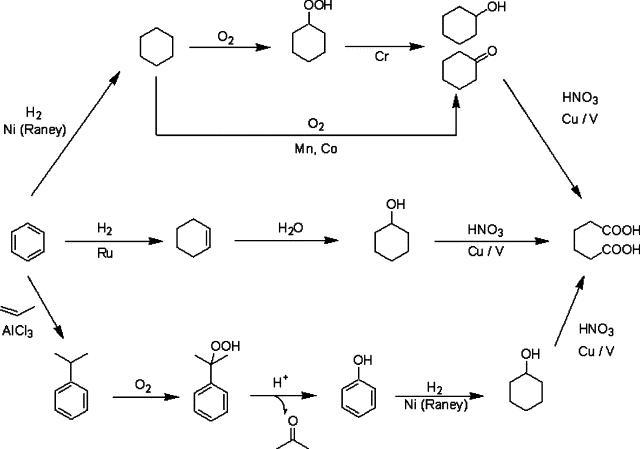
\includegraphics[clip=true,trim=0pt 0pt 0pt 0pt,scale=0.5]{25febi1.jpg}
\caption{Conventional production of adipic acid}
\end{figure}
First 2 steps of process are green in terms of atom economy and involve only addition reactions. Catalysts used in the process can be recycled with minimal wastes. However, conversion of cyclohexanol and cyclohexanone to adipic acid requires HNO$_3$ as an oxidizing agent. The process produces N$_2$O as a byproduct, which contributes to acid rain. A solution can be to recycle N$_2$O to produce HNO$_3$.\\

However, this does not account for the fact that benzene is a petroleum derivative and therefore it is obtained from a non renewable source. In an alternative process, it is replaced by D-glucose, which can be obtained from biomass. D-glucose is treated with E.coli encapsulated in alginate beads, where reaction takes place in solution phase. The efficiency of bioreaction is as high as 98\% and effluent can be filtered to remove bacterial beads.\\
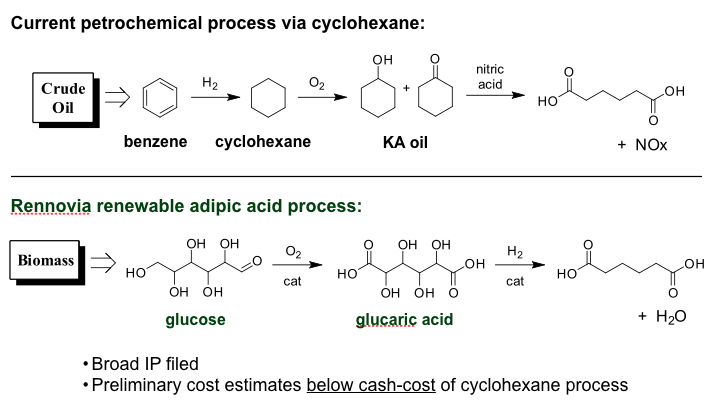
\includegraphics[clip=true,trim=0pt 250pt 0pt 40pt,scale=0.6]{25febi2.png}
\\
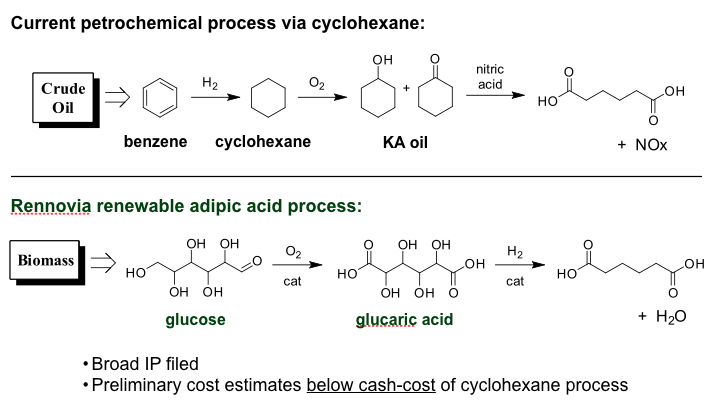
\includegraphics[clip=true,trim=0pt 70pt 0pt 220pt,scale=0.6]{25febi2.png}
\section{Production of Indigo}
Indigo, or indigotin, occurs as a glucoside in many plants of Asia, the East Indies, Africa, and South America, and has been used throughout history as a blue dye. The chemical structure of indigo, corresponding to the formula C$_{16}$H$_{10}$N$_2$O$_2$, was announced in 1883 by Adolf von Baeyer after eighteen years of study of the dye. However, a commercially feasible manufacturing process was not developed until approximately 1887. The method, still in use throughout the world, consists of a synthesis of indoxyl by fusion of sodium phenylglycinate in mixture of caustic soda and sodamide.\\

An alternative process was developed by D.T. Gibson in 1990s, involving biological enzymes. \textit{E.coli} contains the enzyme tryptophanase, which splits the indole group from the peptide backbone. Naphthalene dioxygenase, from the nah operon, then creates a compound which will spontaneously eliminate water and be air oxidized into indigo as the final product. \\
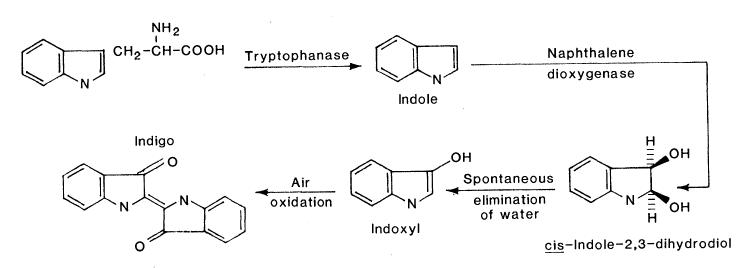
\includegraphics[clip=true,trim=0pt 0pt 0pt 0pt,scale=0.77]{2bfebi3.jpg}
\section{Supercritical Extraction of Caffeine}
\begin{figure}[htb]
\centering
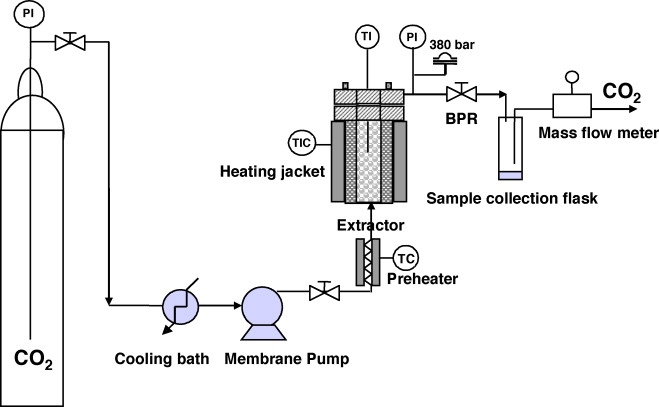
\includegraphics[clip=true,trim=0pt 0pt 0pt 0pt,scale=0.58]{28febi2.jpg}
\caption{Supercritical extraction of caffeine}
\end{figure}
Extraction of caffeine from plant sources is not a green process and utilizes reagents like lead and chloroform. However, the industrial process utilizes supercritical CO$_2$ to leach out caffeine from plant sources. The effluent can be filtered out to obtain a solution of caffeine in CO$_2$. This can be evaporated by releasing pressure, leaving behind a cake of caffeine.
\section*{Conclusion}
For green chemistry, it is not only important to look at atom economy and waste, but also where raw materials are sourced from. The process must also be relatively non hazardous. Further, for the process to be actually implemented, it should not have very high setup costs and must be easy to setup, scale up and operate. If reagents of a plant are changed, new reagents must be compatible with existing plant machinery.
\end{document}